\section{Introduction}
%\label{sec:introduction}
Machine learning (ML) models have been effective at automating various tasks traditionally performed by humans such as character recognition, image classification, sentiment analysis, translation, and fraud detection. For many of these tasks the dataset is not constructed explicitly to provide a training set but has been re-purposed for the ML application. Such datasets may suffer from several challenges: human error in labeling (noisy labels); the labeled set could be not representative of the population (selective labels); and importantly for our application, it could record the labels of only one class (one-sided labels). For example, re-purposing a dataset that documents only criminal convictions (not all trials): the cases tried could be biased (selective labels), and it could also be unknown which cases were tried but did not end in convictions (one-sided labels). In this paper we provide solutions to some of these problems, and others, such as multiple time-period data and in-sample prediction. We do this by developing an important application on a real-world dataset: finding fraudulent firms in the Delhi value added tax (VAT) system.

VAT implementation in many low compliance environments is plagued by firms lowering their tax liability by generating false paper trails. This demand for false paper trails has led to the creation of fraudulent firms that sell fake receipts to genuine firms. These firms are referred to as ``bogus'' firms or ``bill traders'' by the tax authorities. A tax authority usually determines the existence of bogus firms by first filtering down based on a few preliminary indicators, and then undertaking physical inspections that verify if a firm is bogus or legitimate (``legit'' for short). Given the authority's limited resources these inspections are only done sporadically.  While the true revenue implication of bogus firms is unknown, our conversations with tax officials in Delhi (India) suggest that it might be considerable (\$300 million in Delhi alone is a commonly mentioned figure). A key challenge in improving tax compliance then is to regularly, cheaply and reliably identify such fraudulent firms. 

In this paper, we implement and evaluate an ML algorithm on the universe of tax returns data from the Delhi tax authority to identify such bogus firms. The classifier predicts the likelihood of a firm being bogus by using a training dataset comprising the universe of tax returns (over 3 years) and of results from past physical inspections of firms conducted by the tax officials. To our knowledge, this is the first paper to systematically study and identify these fraudulent firms in an economy with weak compliance.

We overcome several non-standard facets of the data and of our problem. First, our dataset was not constructed for the purpose of labeling for an algorithm and is, therefore, not a representative sample of the population. In our case, a small fraction of all firms are inspected, those suspected by the tax authority, and so there is a problem of selective labels \cite{lakkaraju2017selective}. On top of that, the tax authority only records bogus firms that were inspected, caught and canceled, but not firms that were inspected and found to be legitimate. Therefore, we are unable to distinguish between firms that were inspected and found to be legitimate and firms that were never inspected. We refer to this problem as that of one-sided labels, since no firm can be definitively labeled as legitimate (see \cref{fig:onesidedlabel}). The unlabeled firms are (at least weakly) less likely to be bogus than those labeled bogus, and we leverage this difference in class distribution to train a classifier. Moreover, the authority has never identified all the bogus firms in the stock of existing VAT firms, so we want to predict the labels of all unlabeled firms. Therefore, a standard classification approach with a training set and out-of-sample prediction is not viable. We employ a form of cross-validation to use the entire dataset as a training set and make predictions on all firms in the dataset not known to be bogus.

\begin{figure}
  \includegraphics[width=.9\textwidth, page=5]{./figures/StylizedExample_New2.pdf}
  \caption{One sided labels}
  \label{fig:onesidedlabel}
  \floatfoot{\footnotesize Inspection is based on the tax authority's discretion and so are biased (selective labels). Class labels are known only for firms both inspected and found to be bogus, not for the rest (one-sided labels). We use all data for training, but want to predict for those firms still unlabeled.}  
\end{figure}

Second, standard evaluation methods rely on a labeled test set that does not exist in our one-sided labels context. In such a scenario, the task in which the problem is embedded can provide relevant metrics to evaluate the effectiveness of classification methods. In our case, the tax authority has limited resources for inspection and so it will be able to act on only the top model
recommendations. Therefore, it is reasonable to focus on the success of our top recommendations. While considering the performance evaluation results it is important to keep in mind that, according to tax officials, bogus firms are relatively rare (i.e. the class bogus is rare in the population).\footnote{In future work, by  closely documenting the inspection results, we intend to verify this claim.} Our performance estimates remain  valid regardless of the actual prevalence of bogus firms.

Third, in order to compare our algorithm's performance to the status quo of manual targeting for inspection, we carry out what we call point-in-time simulation. We estimate not only whether our model successfully predicts bogus firms, but also whether it would have done better than the tax inspectors themselves. To do this, we test our model's success at a point in time within the span of our dataset. We roll back the data to the state of knowledge at that time and generate predictions. We then measure the performance by using more recent data. In this manner, we can estimate the number of bogus firms our algorithm would have detected before the tax inspectors. We calculate the revenue lost to tax evasion over the period between when our algorithm could have targeted these firms and when they were actually targeted and inspected - potential revenue which we estimate at several billions of rupees (tens of millions of USD).

Finally, each firm files its returns quarterly and so supplies many data points, but its class (bogus or legitimate) is timeless. Therefore, there are several identically-formatted data points for each object of classification (the firm) and classification must be made at the object level. We train a single-period model and aggregate its predictions to the firm level. We call this approach multiple time-period prediction.

The key contributions of our work are:
\begin{compactitem}
\item A novel solution to the classification problem with one-sided  labels, where the labels of many data points are unknown and there  are definite examples only of one class.
\item Point-in-time simulation approach for evaluating real-world prediction systems. We evaluate the impact of our predictions by
  calculating how much our algorithm would have increased collections by identifying bogus firms sooner than the tax authority.
\item An approach for multiple time period (or multiple data-points) prediction, where several data points of similar format exist for each object of classification, but prediction is made at the object  level.
\item An application of machine learning on a large dataset for an emerging economy government to address an important policy problem. Our results indicate that by using our tool the tax administration can prevent fraud up to \rupee1-3 billion (\$15-45 million).
\item A proposed mechanism through which bogus firms may operate in a low compliance, emerging economy.
\end{compactitem}

The remainder of this paper is structured as follows. In \cref{sec:literature} we review the relevant literature both in economics and machine learning. In \cref{sec:vat} we describe the basics of VAT functioning. In \cref{sec:mechanism} we propose the mechanism that we think is behind the existence of bogus firms. \Cref{sec:system-description} describes the classification system we construct. In \cref{sec:evaluation} we evaluate the performance of our system and present the results of our model. Finally, in \cref{sec:2-conclusion} we describe our future goals.


\section{Related Work}
\label{sec:literature}
\subsection{Economics}
\label{subsec:literature-economics}
There is a recent and growing empirical literature on taxation and development. This project fits into a strand within this literature
that explores mechanisms that improve the state's tax collection capacity \cite{khan2016tax}. In contrast to this previous work, we
examine the role of improved information utilization in increasing tax collections. Our paper also fits into a broader literature that seeks to improve government performance \cite{muralidharan2011teacher, glewwe2010teacher}. Whereas this literature emphasizes the role of incentives in improving performance, we hold incentives fixed but instead improve the state's ability to target evasion activity. Our project is also related to a nascent literature on corruption\cite{olken2012corruption, duflo2013truth}. However, rather than relaxing the government's resource constraints (e.g. in terms of inspections), we seek to reduce corruption by improving the state's ability to detect corrupt firms by using technology to better analyze data that is already available to it. Our work also links to the ``forensic economics'' literature which emphasizes hidden behavior in various domains \cite{zitzewitz2012forensic, jacob2003rotten, mironov2014corruption}. We hope to contribute to this literature by identifying features that are predictive of fraudulent firms. Improving the state's ability to tax effectively is increasingly seen as central to the development process and VAT has been proposed as a key tool towards accomplishing this goal.\footnote{See e.g. \cite{besley2013taxation}. See  \cite{Ebrilletal:2001} for an overview of the aggregate cross-country evidence on the effectiveness of the VAT.} Our work also ties in to the emerging literature on micro-empirical investigation of value added tax systems \cite{almunia2017under, mittal2017vat, naritomi2013consumers, pomeranz2015no}.  Although previous work has discussed VAT evasion through fraudulent firms \cite{keen2006vat, pashev2007countering}, this paper appears to be the first to systematically study and identify fraudulent firms in an economy with weak legal and enforcement institutions.

\subsection{Machine Learning}
\label{subsec:literature-ml}
In recent years there has been a growing interest in using ML methods in economic development and in developing countries. These studies cover topics such as measuring poverty \cite{blumenstock2015predicting, xie2015transfer,chen2011using},
population mapping \cite{deville2014dynamic}, migration and mobility \cite{lu2016unveiling}, health and epidemiology
\cite{wesolowski2014quantifying}, financial inclusion\cite{bjorkegren2017behavior}, and program monitoring and evaluation
\cite{wilson2015comparing}. These studies usually harness data sources such as satellite images of luminosity at night \cite{chen2011using}, high resolution remote sensing \cite{xie2015transfer}, mobile phone usage\cite{blumenstock2015predicting, deville2014dynamic, lu2016unveiling, bjorkegren2017behavior}, internet and social media \cite{llorente2015social}, and small digital sensors\cite{wilson2015comparing}. Very few of those studies use proprietary government data, and those that do usually do not have large scale data to benefit from ML and big-data approaches. Furthermore, very few of those studies create a system that can be used by developing country governments directly. To our knowledge, ours is the first study to use ML on large scale tax records from an emerging economy.

\section{Value Added Tax}
\label{sec:vat}
VAT is an indirect tax charged at multiple stages of production (and distribution) with taxes paid on purchases (inputs) credited against taxes withheld on sales (output). Firms withhold taxes on sales (output tax) from which they deduct the taxes they have already paid on purchases (input credits), and finally remit the difference to the tax authority. Thus, unlike under a retail sales tax, the tax authority collects tax revenue throughout the production chain. The VAT system also requires both firms involved in a transaction to report it independently allowing the tax authority to verify sale declarations of the seller against buyer reports while inspecting returns, known as third party verification.\footnote{See \cite{ITD2005} for more details.\cite{mittal2017vat} further describes VAT compliance incentives, and evaluates a technology implementation intended to improve compliance in Delhi. }

In \cref{fig:bogus-mechanism}, we illustrate a simple VAT chain assuming a uniform tax rate of 10\%. Firm A sells goods worth \$60 to firm C. Firm C sells it ahead to Firm D at a price of \$80. Firm D finally sells to an end customer at the price of \$90. In this example, the tax authority collects tax on \$90 of value added (\$9 of tax at tax rate 10\%). \$60 of the value add (\$6 tax) comes from firm A, \$20 of the value add (\$2 tax) comes from firm C, and \$10 of the value add (\$1 tax) comes from firm D. Third-party verification works in the following manner. All firms have to report transaction level information. Firm C wants to report that it made a purchase of \$60 from firm A as that report reduces the tax that it would have to remit to the tax authority. As a result, firm A would also have to declare the sale of \$60 and subsequently pay the tax on it. Similarly, firm D will make firm C report the sale of \$80.

\begin{figure}
  \includegraphics[width=1\columnwidth, page=2]{figures/StylizedExample_New2.pdf}
  \caption{Stylized example illustrating a value added tax transaction chain}
  \label{fig:bogus-mechanism}
\end{figure}
However, genuine firms may want to bypass the constraints imposed by third-party verification by reporting fraudulent transactions with bogus firms. Given the attention that governments in emerging economies have begun to pay to ``ease of doing business'' norms, registering a firm is increasingly straightforward. These factors have led to the emergence of bogus firms. In \cref{sec:mechanism}, we explain the possible mechanism through which these bogus firms operate and lead to tax evasion.

\section{A Mechanism of Bogus Firms}
\label{sec:mechanism}
We now propose a mechanism that allows bogus firms to operate over multiple periods. In \cref{fig:bogus-mechanism2}, we build on the stylized example by introducing the bogus firm B. The new transactions take place only on paper (i.e. are fraudulent). The actual transfer of goods stays the same as described  in \cref{fig:bogus-mechanism}. Firm D diverts \$40 out of the \$90 business-to-customer sales that it was actually making to the final consumer to firm B and reports it as a business-to-business sale.\footnote{Firm B may make a side payment to firm D as a small kickback for violating the law by misreporting. }  Firm D can do this because it makes sales to final consumers who are not incentivized to provide reports of such transactions to the tax authority, and because this does not increase financial liability of firm D to the tax authority.  

Firm B then can sell the input credit it now has to firm A by showing a sale of an amount weakly greater than \$40 to firm A. The value add of firm A is now \$19 instead of the true value which should be \$60.\footnote{Firm A will be willing to make significant payments to firm B as this reduces firm A's tax liability.} Value added by bogus firm B is \$1, and firm C and firm D have the same value added as earlier. The final value added in the system now is \$40 less relative to a fully compliant system. The surplus (tax evaded) can potentially be divided between the offending firms, i.e. A, B (bogus), and D.

A few key observations need to be highlighted. First, firm A and firm D do not need to be in the same transaction chain. It is not necessary for the eventual chain of transactions to be circular. Firm C does not benefit from the bogus transactions and need not even know about them.\footnote{We include firm C to highlight that such transactions can co-exist around genuine transactions.} Second, bogus firm B can make sales to any firm which is in need of input credits. It does not necessarily need to make such sales to firm A which is at the beginning of the transaction chain. Third, we believe that once detected it is not complicated to verify that firm B is bogus. It is a fake firm which should not exist physically at the address submitted to the tax authority.\footnote{In subsequent field work we can test this assumption} Therefore, there is no need to rigorously analyze its business related paperwork (high effort) and a visit to the location (relatively low effort) should be sufficient. Finally, after identifying bogus firm B, the revenue can only be recovered if the authority pursues firm A and reverses the input credit that firm A has claimed. Any kind of a penalty only on firm B does not recoup the revenue loss. We now describe the design of our system.

\begin{figure}
  \includegraphics[width=1\columnwidth, page=4]{figures/StylizedExample_New2.pdf}
  \caption{An example showing how bogus firms facilitate tax evasion}
  \label{fig:bogus-mechanism2}
  \floatfoot{\footnotesize Firm A and Firm D need not necessarily be in the same chain. Bogus firms can make sales to any firm which needs input credits.}
\end{figure}

\section{System Description}
\label{sec:system-description}
\subsection{Data}
\label{subsec:2-data} 

Our dataset has almost 3 years of quarterly VAT returns from the National Capital Territory of Delhi, India from 2012-13 to 2014-15 (with personal identifying information removed). This includes consolidated returns as well as transaction level information filed by an unbalanced panel of firms, $|Firms|=315,191$, and a list of firms that were previously found to be bogus by the tax authority, $|inspected \& bogus|=538$.  Returns are filed quarterly so we should ideally have data from 12 quarters. However, for the fourth quarter of 2012-13 the transaction level records are unusable and therefore we drop that quarter from our analysis, which leaves us with data from 11 quarters. We denote these as follows. $Returns_{f,t}$ for firm $f\in Firms$ in quarter $t \in Q(f)\subseteq Q \equiv \{1,2,3,5,...12\}$, where firm $f$ operated in quarters $Q(f)$ (t=4 was dropped). Every firm is either bogus or legitimate and this doesn't change over time:$class_f \in \{bogus,legit\}$.\footnote{This is an assumption, but we have good reason to believe it from discussions with the tax authority and since there are sanctions against owners of bogus firms that are found, so owners would not use their legitimate companies for this purpose.} Some firms were inspected: $inspected_f \in \{True,False\}$ and of those inspected some were bogus and some legitimate, but this is recorded in our data only for the ones that were found to be bogus.\[ label_f =y_f= 
     \begin{cases}
       \text{bogus,} &\quad\text{if $inspected_f$ and $class_f=bogus$} \\
       \text{unlabeled,} &\quad\text{if $inspected_f$ and $class_f=legit$} \\
       \text{unlabeled,} &\quad\text{if not $inspected_f$} \\
     \end{cases}
\]

When a bogus firm is inspected at time T, it is caught and stops operating, $max(Q(f))=T$. Due to confidentiality concerns, the personally identifiable information has been removed and each firm is assigned a unique identifying number so that we can follow a firm over time as well as track its presence in other firms' returns. However, we cannot link the returns to any other publicly available information on the firms. We have detailed information on the line items in the consolidated returns, $Returns_{f,t}$, as well as line items from annexures, $Transactions_{f,t}$, where each firm reports the total purchases it made from (and sales to) each other firm at each tax rate level for that quarter. 

In addition to tax return information we also have access to basic information provided by the firm at the time of registration, $Profile_f$. Firms are mandated to keep this information updated. We observe the date of registration, the revenue ward (broad geographic location of the firm), the nature of business (e.g. manufacturer, wholesaler, retailer), its legal status (e.g. proprietorship, private limited company), the other tax schemes and acts it is subject to (e.g. central excise act) and whether it is registered for international trade (import or export).

\subsection{Features}
\label{subsec:features}
Our unit of observation is the firm-quarter level. We have an observation for each firm in each quarter in which it filed a return: firm A in quarter 1, firm A in quarter 2, firm B in quarter 1, firm B in quarter 2, etc. We ensure that none of the features use data from different time periods - they are all within the quarterly observation. We detail them in this section. In \cref{subsec:multi-period} we describe how we use the firm-quarter level observations to make predictions at the firm level.

Some of our features rely on domain expertise or anecdotes from the tax authority. For example, ``VAT/Turnover ratio'' is the ratio of tax paid to total turnover. To illustrate why this feature might be predictive, in \cref{fig:bogus-mechanism2}, if firm B reported value add of \$2 instead of \$1, it would have to pay VAT for that added dollar and will also have to reduce firm A's fake input credits by \$1. Firm B is not actually carrying out any trade, and is relying on the arbitrage between firm D and firm A to make money. This implies that it wants to minimize its declared value add or, equivalently, have a low ratio between tax paid (proportional to profit) and total turnover. 

Another example of a feature we hypothesize to be predictive is the proportion of sales a firm makes to unregistered firms - these could be small firms that are not subject to reporting or they could be final customers. An unregistered firm does not claim input credits and so cannot benefit from the services of bogus firms. We would accordingly expect bogus firms to report selling a very small share of their sales to unregistered firms, and this is borne out in our (admittedly selected) data.
Our features can be divided into 3 broad sets: $X_{f,t}=featureExtraction(Profile_f, Returns_{f,t},Transactions_{f,t})$. First is the set of profile features which come from the registration information provided by the firms. The second set of features come from the quarterly consolidated returns that each firm has to file. These include variables such as total turnover, within-state turnover, the amount of VAT that was actually paid, etc. 
Finally, the third set of features come from the annexures that firms have to file along with the consolidated returns.\footnote{Based on our interactions with various tax officials, tax administrations in general do not have the capacity to rigorously use the transaction level information that is now available to them. They mostly use it only for third-party verification purposes.} These annexures cross-reference the firm's declarations of their transactions, who it sold to, and how much that other firm reported buying back. Using these annexures, we create variables such as discrepancies in reporting between clients and suppliers, the weighted VAT/Turnover ratio of client firms, the weighted VAT/Turnover ratio of supplying firms, share of sales made to biggest client, and network features such as PageRank etc. 

We refrain from using the class labels of neighbors in the network in our features because it would compromise the estimates of performance by creating leakage between training and test set, and also because we would need a point-in-time simulation to train this, since only the class labels of firms caught before a certain time period can be used as a feature when training for that time period, otherwise we create leakage from the future to the past. 

\subsection{Class Labels}
\label{subsec:class-labels} 
In this section we describe how class labels are constructed from our data, and the problems this poses.

\subsubsection{Selective Labels - Biased Training Set}
\label{subsubsec:biased-training-set} 
The labels in our training set come from a list of firms that were targeted for inspection by the tax department, inspected, found to be bogus, and subsequently had their registration canceled. This procedure creates a biased training set as the firms targeted for inspection are not random - in fact they were chosen explicitly by the tax department as suspicious of being bogus, so are not representative of the general population (see \cref{fig:onesidedlabel}). This is the selective labels problem \cite{lakkaraju2017selective}.  We do not have a way of completely eliminating the effect of this bias on performance. However, we \textit{evaluate} our performance in a way that produces bounds which are not affected by this bias. In the future we plan to carry out inspections based on our model's predictions, which would provide an unbiased performance estimate.

\subsubsection{One-sided Labels}
\label{subsubsec:one-sided-labels} 
A more serious problem with our labels is that among the inspected firms we do not have records of which firms were found to be \textit{legitimate}, and so not canceled. This is because the tax authorities do not keep records of which firms were inspected, only which ones were found to be bogus and canceled. In our data, we are unable to distinguish the legitimate but inspected firms from those never inspected. Our labels are thus one-sided: we have firms that we know to be bogus - those canceled, and firms that we do not know for sure but are likely to be legitimate - all the rest. To further clarify the difference between selective and one-sided labels, if the tax authority randomly sampled firms for inspection, this would solve the selective labels problem but the labels might still be one-sided if they only recorded the firms found bogus.

The unlabeled firms are likely legitimate since the base rate of bogus firms in the population is not very high, though we do not know it precisely. However, they are not all legitimate as evidenced by many firms in the data being caught as bogus only after operating and facilitating tax evasion for many quarters. Therefore, we do not have a labeled training set (see \cref{fig:onesidedlabel}). This is related, though not the same, as the problem of classification with noisy labels \cite{liu2016classification, natarajan2013learning}.

We define classes for all our observations in the following way. In our outcome variable, we classify firms that were found to be bogus as 1 (``bogus'') and the rest of the firms, whether never inspected or those that were inspected, found to be legitimate and not recorded, as 0 (``probably legit''). This is an acceptable starting point as bogus firms are rare in the unlabeled set. These are two classes so it seems we can solve a standard classification problem but that is not the case. There is no out-of-sample prediction to be made on some other firms that are not already labeled by this process. We are interested in predictions on the ``probably legit'' firms, since some of them may actually be bogus and we would like to target them for inspections. We will detail our solution in \cref{subsec:cvp} and \cref{sec:evaluation}. While our classifiers would fit to predict inspected and bogus firms (selective labels), as in our training data, these are nonetheless bogus firms that they are finding. Additionally, even training on the selective set, the classifiers might learn from features not used by the tax officials and improve performance for all bogus firms.

\subsubsection{Multiple Time Periods}
\label{subsubsec:multiple-time}
For each firm, the class does not change over time - a firm does not start legitimate and become bogus, or the other way around. However, a firm is supposed to file a return every quarter. We use our classification of firms to classify all quarterly observations of that firm with the class of the firm: ``bogus'' or ``probably legit''. $y_{f,t}=y_f \in \{bogus,legit\}$.


\subsection{Classifier}
\label{subsec:classifier}

\begin{figure}
  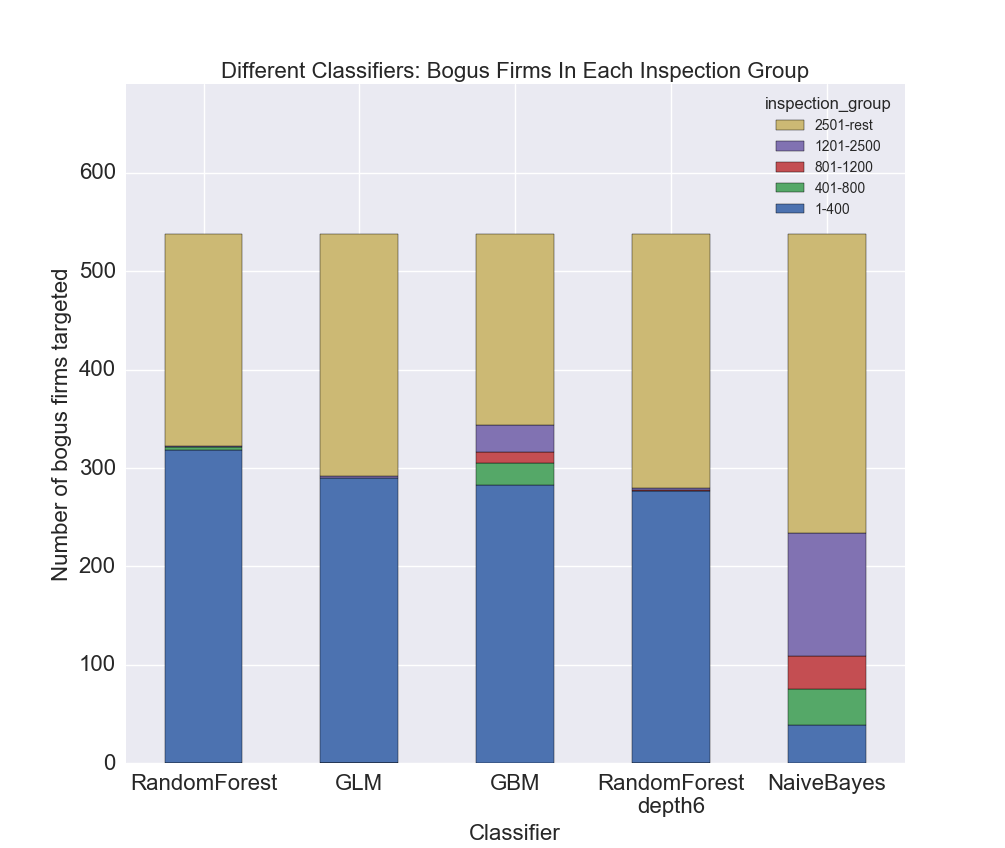
\includegraphics[width=0.4\textwidth, page=1]{figures/DifferentClassifiersPerformanceByInspectionGroup.png}
  \caption{Comparison of Different Classifiers}
  \label{fig:differentclassifiers}
\end{figure}

We use a Random Forest \cite{liaw2002classification} classifier with $n\_trees=200$,\\ $stopping\_rounds=2$, and $max\_tree\_depth=20$ (the maximum depth is rarely reached in practice since the tree bifurcation stops when too few classification examples are left in a leaf) in H2O python implementation \cite{h2o_Python_module}. We selected Random Forest for its ability to handle complex dependencies between features (since not all our features are independently predictive) and combine categorical variables together with continuous variables seamlessly. 

We perform a comparison of the performance of different classifiers to see if our results are sensitive to the choice of classification algorithm. \Cref{fig:differentclassifiers} shows our results: a few  standard classification algorithms obtain similar performance. For the top 400, 800 or 1200 recommendations Random Forest performs best. The one algorithm which performs worse than others is Naive Bayes, which is unsurprising since many of the features we use are not independent and since the algorithm implementation we used also assumes Gaussian distribution for numerical features conditional on class \cite{h2o_NaiveBayes}, which does not hold with our numerical features.

\subsection{Cross-Validated Predictions}
\label{subsec:cvp}
\begin{figure}
  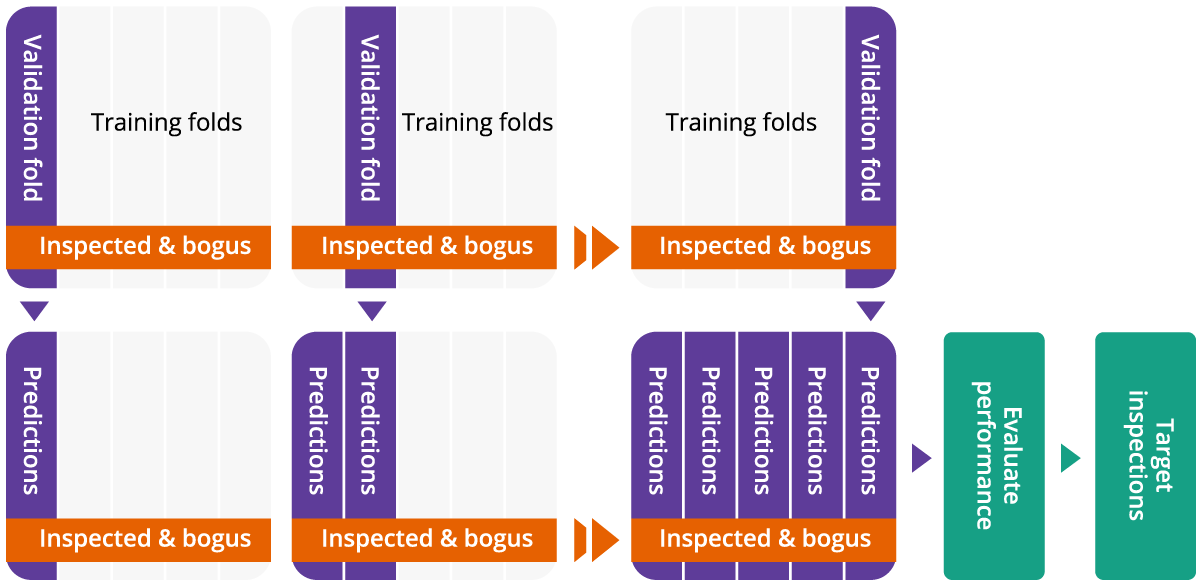
\includegraphics[width=1\columnwidth]{figures/CrossValidatedPrediction.png}
  \caption{Cross-validated prediction procedure}
  \label{fig:crossvalidation}
\end{figure}

We have preliminarily classified all our dataset to ``bogus'' and ``probably legit'', as explained in the \cref{subsubsec:one-sided-labels}, and so it would seem that there is no more need for in-sample predictions to target inspections. However, for our real-world application, we want the model to help target inspections of existing unlabeled firms. Of the firms we classify as ``probably legit'', some are bogus and we want to find them. If we trained a classifier on all the observations (classes ``bogus'' vs. ``probably legit'') and then made predictions on the ``probably legit'' firms, we would be overfitting as a result of leakage since our model would train on certain examples and then be used to make a prediction on one of those same examples. This problem comes up in cases of prediction using noisy labels, where it is required to make predictions on the noisily-labeled data that is used for training.

To avoid this, we carry out cross-validated holdout predictions. We randomly divide our data into 8 folds. We also ensure that all quarterly observations of a firm are within the same fold, which is crucial to avoid a different type of leakage across time-periods. Formally, for each firm we draw a fold: $fold_f \in \{0,1,2,...,7\}$. We divide our data into these folds: $Fold_j = \{(X_{f,t},y_f) \space | \space f \in Firms,\space t \in Q(f), \space fold_f=j\}$. We generate predictions for all of our sample by performing 8-fold cross-validation: train on 7 folds with classes ``bogus'' vs. ``probably legit'' and make predictions on the remaining fold. We then save those holdout predictions for all of the folds - for each fold from when it was the validation fold. In this way we generate predictions for our entire dataset (see \cref{fig:crossvalidation}). To obtain predictions for firm $f$:
\begin{enumerate}
\item $\text{Train on all other folds: } Model.train(\bigcup_{j\neq fold_f} Fold_j) $
\item $\text{Make prediction: }\hat{y}_{f,t} = Model.predict(X_{f,t}) $
\end{enumerate}

To evaluate performance, we will compare those predictions $\hat{y}_{f,t}$ to the known classes $y_f$ (see \cref{sec:evaluation}). To target inspections, we plan to discard predictions for firms that are known to be bogus (since they were already canceled), and focus on the ones remaining with the highest model-predicted likelihood of being bogus. 

More than 8 folds would make for better predictions, but increase computational expense. Increasing the number of folds from 8 to 16 would increase the size of the training set from 7/8 to 15/16 - an increase of 7\% - but more than double the computation time. The extreme ideal for prediction would be leave-one-out, which would be computationally unfeasible on our dataset. Our method is not specific to the context of bogus firms, but can be used in any scenario with noisy labels and in need of in-sample prediction. 

\subsection{Multi-Period Model}
\label{subsec:multi-period}
Each firm operates and files returns every quarter, and so we have multiple observations for each firm $f$ - one for each quarter - with different feature values $\{(X_{f,t},y_f)\space | \space t \in Q(f)\}$. However, a firm is either bogus or not and this does not change with time, so predictions should be made for a firm, $\hat{y}_f$, not a firm in a specific quarter, $\hat{y}_{f,t}$. So we need to consider these different feature values but produce one prediction per firm. We do this in three steps. First, we train a single-period model on firm-quarter observations. Second, we use the single-period model to make predictions for all firm-quarter observations, $\{\hat{y}_{f,t}\}$. Third, we aggregate the firm-quarter predictions to the firm level to produce a single prediction per firm, $\hat{y}_f=Aggregate(\{\hat{y}_{f,t}\space|t \in Q(f)\})$ (see \cref{fig:aggregation}). For generality, we describe this situation as if we have full labels and separate $trainingSet$ and $testSet$, but we combine this approach with our approach for one-sided labels.

\begin{figure}
  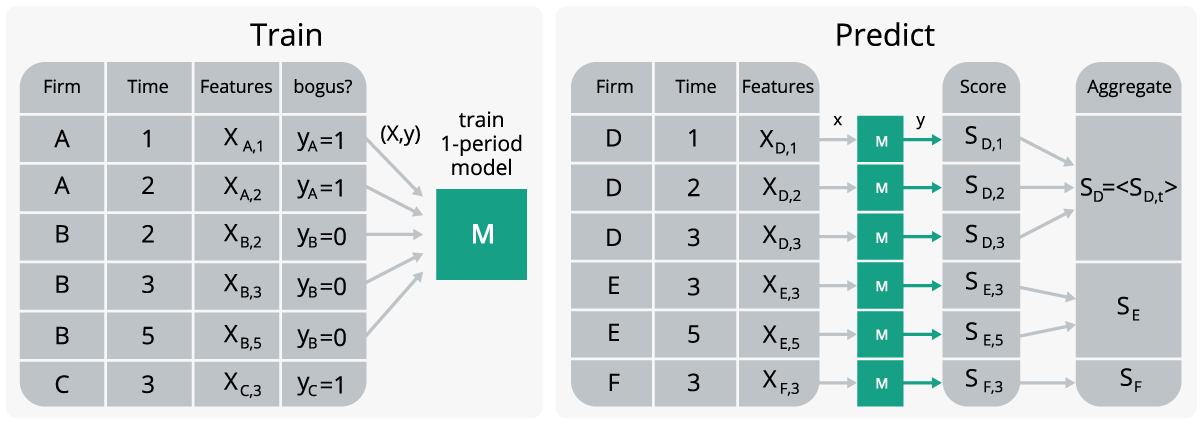
\includegraphics[width=1\columnwidth]{figures/MultiplePeriodPrediction.png}
  \caption{Generating firm level predictions from firm-quarter level data points}
  \label{fig:aggregation}
\end{figure}

\subsubsection{Single-Period Model}
\label{subsubsec:single-period-model}
Each firm  $f$ has multiple firm-quarter data points, all classified according to the class of that firm. We use all these points to train a single-period model: \[Model.train(\{(X_{f,t},y_f) \space | \space f \in trainingSet\})\] In our case, $trainingSet$ is simply all folds other than the one to which firm $f$ belongs. Rather than taking only one observation per firm or re-weighting them so that each firm has equal total weight, this model is unaware of the fact that different observations belong to the same firm (or to different quarters) and treats them all independently (see left panel in \cref{fig:aggregation}).  This might affect performance depending on the behavior of the same firm in different quarters and how much marginal information each observation adds to the classification problem. If features in different quarters by the same firm are identical, then our procedure only introduces unbalanced duplication. If they are different, then different time-periods add valuable training examples that are all separate pieces of evidence for what bogus firms look like and our procedure is justified. Our procedure may also result in biased data based on whether firms were caught early or late, since those caught later operate in more quarters and so have more data points on which to train on and would influence the classifier more.

\subsubsection{Single-Period Predictions}
\label{subsubsec:single-period-prediction}
We use our single-period model to make predictions on firm-quarter observations: \[\hat{y}_{f,t}=Model.predict(X_{f,t})\] The model is unaware of the fact that different observations may belong to the same firm. These predictions are model-predicted probabilities of being bogus - numbers between 0 and 1, where 1 is certainty of being bogus, and 0 is certainty of being legitimate. In this way we generate predictions for all the observations, using for each firm all folds that do not contain that firm as described in \cref{subsec:cvp} (see right panel in \cref{fig:aggregation}).

\subsubsection{Aggregating Predictions to The Firm-Level}
\label{subsubsec:predictionaggregation}
Eventually, we want to make a single prediction for a firm by combining the information available across quarters. We do this by aggregating the single-period model-predicted probabilities at the firm level to create final predictions (see \cref{fig:aggregation} right panel): \[\hat{y}_f=Aggregate(\{\hat{y}_{f,t}\space|t \in Q(f)\})\]

We experimented with different functions for aggregating single-period predictions. For example, if a firm's single-period predictions were 0.1, 0.2, 0.6 then the arithmetic mean aggregating function would produce a score of $0.3$, whereas the maximum aggregating function  (maximum model-predicted probability of being bogus across periods) would produce $0.6$. In practice, the arithmetic mean works best, only slightly ahead of the maximum score function. We therefore end up using the arithmetic mean as our aggregating function. Other functions that we tried were ``take the score of the first (last) period for that firm'', and ``maximal (minimal) score for that firm across all periods''.  

There are other approaches that can potentially address the multiple time period problem. For example, aggregating the features before generating predictions instead of aggregating predictions, or treating each firm as a single observation and the list of its quarterly VAT returns as the corresponding feature vector. All approaches have their own challenges and we picked the one that we seemed least problematic. If we aggregate feature values before generating the predictions, we might end up losing the variation in  multiple observations of the same feature. If we combined all quarters to ensure that each firm had a single observation, then the same feature across time will be treated independently, so in effect we’re reducing the number of points in the training set. Moreover, entry and exit of firms in different time periods will result in the dataset having a lot of NULL values.

Our chosen approach is not specific to multiple time periods. It is applicable whenever there are several identical-format data points for each object of classification (the firm, in our case) but classification must be made at the object level. For example, different doctor visits per patient,  or fraud detection based on multiple online purchases by the same customer, or many monthly behaviors of the same object.

\section{Evaluation of Performance}
\label{sec:evaluation}
\subsection{Top Recommendations}
\label{subsec:top-recommendations}
We are constrained by the number of firms the tax authorities can physically inspect, and so we aim to provide a ranked list of suspicious firms. Performance on other parts of the distribution has no real world implications. We rank our firms in descending order of model-predicted likelihood: $rank(f1) \leq rank(f2) \text{ iff } \hat{y}_{f1}\geq \hat{y}_{f2}\text{.  } rank(f) \in \mathbb{N}$. We take a few realistic numbers of top recommendations and check our model's success on those - of these top $N$ firms predicted to be bogus by our model, how many are known to be bogus? Formally, $\text{bogus in top N}=|\{f\space|\space rank(f)\le N,y_f=bogus\}|$. 

Of our top 400 most suspicious firms, we find 75\% to be actually bogus. Of the next 400 - 12\% are actually bogus. Of the next 400 - 6\%, of the next 1300 - 3\%, and of the general population - a negligible fraction (see \cref{tab:AllTimeCVPerformance}). Our model finds more than 75\% of firms labeled ``bogus'' in the top 2,500 recommendations - less than 1\% of firms, which is very good performance. Moreover, recall that the ``probably legit'' firms in this dataset are not necessarily legitimate - they could be bogus unknown to us because they were not inspected - so these numbers for the true-bogus rate in $N$ inspections are underestimates. See \cref{fig:AllDataPerformanceTop1000} for more fine-grained results on the top 1000 recommendations.


\begin{table}
  \begin{tabular}{lrrr}
  	\toprule
	  {\small\textit{Inspection}}  & {\small\textit{Firms}}  &  {\small\textit{Total Bogus}}  &  {\small\textit{Bogus Firms}} \\
    {\small\textit{Group}} & {\small\textit{Inspected}} &{\small\textit{Firms Caught}} & {\small\textit{Caught/Inspection}}\\
    \midrule
              1 - 400 &              400 &                     305 &                           0.76 \\
            401 - 800 &              400 &                      48 &                           0.12 \\
            801 - 1200 &              400 &                      24 &                           0.06 \\
          1201 - 2500 &             1300 &                      29 &                           0.02 \\
          2501 - rest &           313229 &                     132 &                           0.00 \\
    \bottomrule
  \end{tabular}
  \caption{Model performance on top recommendations}
  \label{tab:AllTimeCVPerformance}
  \floatfoot{\footnotesize Using data from all time periods and cross-validated predictions.}
\end{table}
 
\subsection{Top Recommendations - Maximizing Revenue}
\label{subsec:top-recommendations-revenue}
From tax authority's perspective, we want to maximize expected revenue captured, and not merely the likelihood of finding a bogus firm. Small firms will only account for a small amount of tax evaded, and larger bogus firms will account for a much larger amount.\footnote{More precisely, this is determined by the amount of tax input credits claimed, the \$40 in the stylized example above.} We would therefore want a different ranking, in descending order of expected recovered revenue and not of model-predicted likelihood of being bogus. We use the following procedure to make such recommendations.

\begin{figure}
  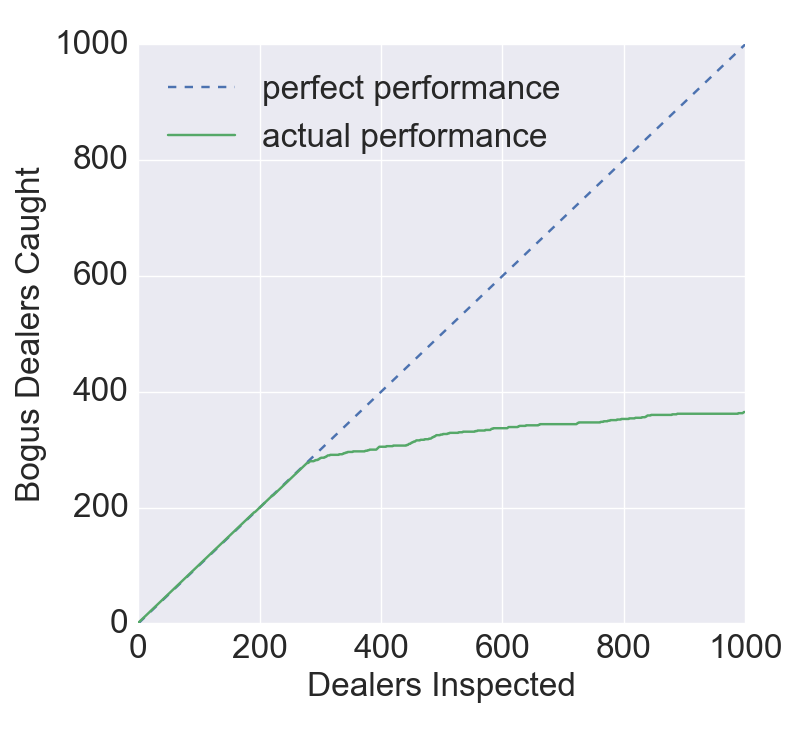
\includegraphics[width=0.35\textwidth]{figures/PerformanceAllData_v2.png}
  \caption{Model performance on top 1000 recommendations}
  \label{fig:AllDataPerformanceTop1000}
  \floatfoot{\footnotesize Using cross-validated predictions on all time periods. The x value is the rank N of suspicious firms and the y value is the number of firms out of those N that are bogus. The dashed y=x line indicates perfect performance, i.e. every firm inspected is bogus. Model performance is near-perfect for the first 250 predictions, then starts to level off.}  
\end{figure}
First, calibrate the model, so its score is an unbiased estimate of the actual probability of being bogus: $E[y_f|\hat{y}_f\approx a]\approx a$. For example, of firms with model score of 0.1, about 1 in 10 should be bogus, for those with model score  0.01 about 1 in 100 should be bogus, etc. This is not automatically the case for predictive models (e.g. Naive Bayes, which tends to extremes with more and more dependent features). Our model turns out to be very well calibrated (results not reported).

Second, calculate expected revenue recaptured by taking the amount of input tax credits the suspicious firms claim (as depicted in \cref{fig:bogus-mechanism2}) as the lost revenue to be recaptured, and multiplying it by the calibrated model score as the probability of a firm being bogus: $ExpectedRevenue_f=\hat{y}_f\cdot InputCredits_f$. We then rank all firms in descending order of the expected revenue captured, and recommend the top ones. On our data the performance of this method in terms of revenue is comparable to the earlier described method and therefore we do not report the results.

\subsection{Different Feature Sets}
\label{subsec:feature-sets}
We have constructed 3 distinct feature sets which we use together in our model: features constructed from the individual firm's returns ($Returns_{f,t}$), features constructed from the firm's dealer profile ($Profile_f$), and features constructed from the network of firms and their trading partners ($Transactions_{f,t}$). We now disaggregate those feature sets and evaluate the performance of the model with each possible combination of feature sets. See \cref{fig:AllDataPerformanceDifferentFeatureSets} for the results. There is a three-way tie between feature sets that contain $Profile_f$ and one other feature set, so that the addition of the third one makes no discernible difference.

\begin{figure}
  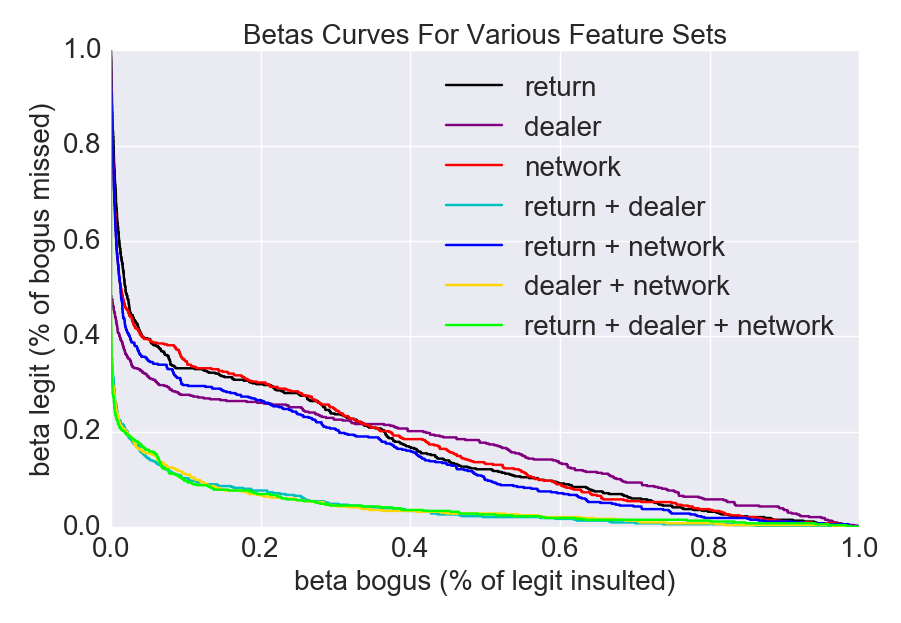
\includegraphics[width=0.4\textwidth]{figures/PerformanceDifferentFeatureSets_v3.png}
  \caption{Betas curves for different feature sets}
  \label{fig:AllDataPerformanceDifferentFeatureSets}
  \floatfoot{\footnotesize The beta curve is 1 minus the ROC curve. As we vary the classification threshold, the x value tracks the fraction of ``probably legit'' firms that will be insulted by getting inspected ($\beta_{bogus}$); the y value tracks the fraction of bogus firms that will be missed by being classified as legit ($\beta_{legit}$). A lower curve indicates better performance.}
\end{figure}

\subsection{Point In Time Simulation}
\label{subsec:PITSimulation}
Our performance estimates so far may seem unrealistic. If we use our model in a real-world scenario, we will not have access to all returns by all firms and will not be required to predict retroactively which firms were caught as bogus and which were not. In a realistic scenario, we would have the returns of all firms up to a certain point in time, and would have to predict which of the firms still operating are likely to be bogus and need to be inspected. Some of those inspected would actually turn out to be bogus. We therefore propose another metric to gauge our performance: point-in-time simulation. 

We build a model based on the state of knowledge and data at a certain point in time T, when the returns for quarter T have been filed but inspections between quarters T and T+1 were not yet performed. We blind our model to all information in the dataset obtained after time T - we do not consider ``future'' tax returns of firms from times greater than T. For our training purposes we only use firms that had already been classified as bogus and canceled by time T. This means that bogus firms caught after time T are classified in the training set as legit. We argue that this strategy simulates the state of knowledge and data at time T (\cref{fig:PointInTimeSchematic}, a panel describing T=3).
\[SimulationTrainingSet_T = \{(X_{f,t},\tilde{y}_{f,T}) | t\le T\}\]
\[   
\tilde{y}_{f,T} =
     \begin{cases}
       \text{bogus,} &\quad\text{if $y_f=bogus$ and $max(Q(f)) \le T-1$} \\
       \text{legit,} &\quad\text{if $y_f=bogus$ and $max(Q(f)) \ge T$} \\
       \text{legit,} &\quad\text{if $y_f=legit$} \\
     \end{cases}
\]
\[SimulationTestSet_T = \{(X_{f,t},y_f) | t\le T,max(Q(f)) \ge T\}\]

\begin{figure}
  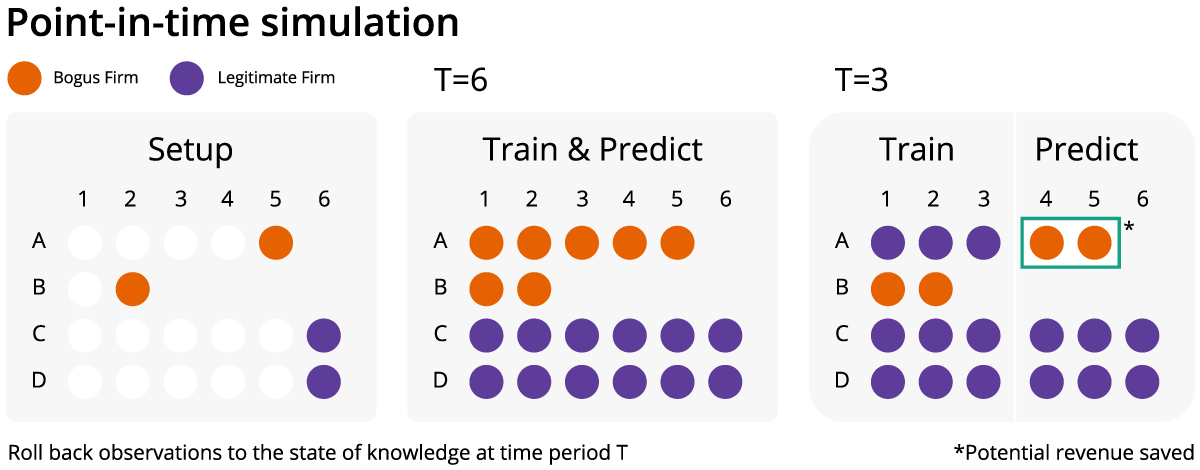
\includegraphics[width=1\columnwidth]{figures/PointInTimeModel.png}
  \caption{Illustration of point-in-time simulation at T=3}
  \label{fig:PointInTimeSchematic}
\end{figure}

We then run our prediction algorithm on this state of the data to generate top recommendations for firms still operating at time T. We evaluate performance by using, for the validation set, the real class of firms which were later caught as bogus ($y_f=bogus$ and $max(Q(f)) \ge T$). Allotting $N$ inspections based on our simulated model's top recommendations, we determine the number of bogus firms, which were later caught by the tax authorities, that our model would have ranked in the top $N$ in time $T$. By summing the input tax credits that these recommended bogus firms claim in time periods greater than T, we can estimate how much lost revenue could have potentially been saved by using our model.

For example, suppose there are 4 firms: A, B, C, D and 6 time-periods as in \cref{fig:PointInTimeSchematic}. Firm A was inspected and identified as bogus in t=5, and firm B was inspected and identified as bogus in t=2. At T=6 after all returns have been filed and inspections have taken place, we know the class of all firms and so we know that firms A \& B are bogus. Our previous performance estimates use this state of knowledge to train, predict and evaluate performance (T=6 panel). 

Now when we simulate the state of knowledge at time T=3, we would have our features for t=1,2,3. We would also know that firm B is bogus, since it was caught and canceled after quarter t=2 and so did not file a return in quarter t=3. However, we would not know that firm A, which would be caught and canceled after quarter t=5, is bogus, and so it would be labeled as ``probably legit''. Firms C \& D would also be labeled as ``probably legit''. We now train our model on all observations from t=1, 2, 3. We use these observations to make predictions on firms A, C, D but not on firm B - since it was already canceled and is no longer operating so there is no point in targeting it for inspections. Suppose that firm A is targeted for inspection based on its features in t=1, 2, 3. We can now discern ourselves to its real class, ``bogus'' - in reality only discovered at t=5, and see that we correctly identify it as bogus in T=3. If we were to conduct inspections based on these recommendations, firm A would not have been able to operate in periods 4 and 5, and the tax evasion it facilitated in those periods would have been avoided and revenue loss averted (\cref{fig:PointInTimeSchematic}, T=3 panel, marked by asterisk). 

This assumes no substitution, i.e. that if a firm was using the services of a bogus firm to evade taxes and that bogus firm is caught and canceled, then the client firm does not find another bogus firm to facilitate its tax evasion but instead pays the required tax. We intend to rigorously test to what extent this is the case in future work using a randomized controlled trial. To adjust our revenue implications to substitution, we can multiply the revenue captured by a factor between 0 and 1 indicating what fraction of the evasion was not substituted.

Results of point-in-time simulations for various times T are detailed in \cref{tab:PointInTimeResults} and plotted in \cref{fig:PointInTimePerformanceArea}. Even based on only a few time periods, our simulated model succeeds in targeting a sizable fraction of bogus firms in the first 400 inspections (0.12\% of firms). Almost all bogus firms targeted by the model fall in the top 400 recommendations, with the other recommendations contributing very little. The performance improves when time advances from T=2 to T=4 since the model has more labels for training (labels from t in \{1,2,3\} vs. \{1\}), but then declines towards the end of the dataset when there are not many bogus firms left to be detected. Note that these simulations are not disjoint - many of the firms we would have caught in T=2 are the ones we would have caught in T=4, 6 and so on. So we cannot simply add up the numbers of firms caught and revenue captured, but have to select one. Of course, these are underestimates since some of the most suspicious ``probably legit'' firms are in fact bogus firms that were never inspected.

The number of bogus firms caught and the revenue saved are also calculated per inspection, showing an excellent hit rate of about 1 in 3 and extremely high returns for the first 400 inspections.  In all, the top 400 recommendations catch between 20\% and 40\% of all known bogus firms operating at that time.

\begin{table*}
  \begin{tabular}{rrrrrrr}
  	\toprule
	  &&& {\small \textit{Revenue Gained}}& {\small \textit{Revenue Gained}}&&{\small \textit{Revenue Lost}} \\
    & {\small \textit{Total Bogus}} &{\small \textit{Bogus Firms}}&{\small \textit{by Inspecting}}&{\small \textit{per Inspection}}&{\small \textit{Total Bogus}}&{\small \textit{from All Bogus Firms}}\\
  {\small \textit{T}}&{\small \textit{Firms Caught}}& {\small \textit{Caught/Inspection}}&{\small \textit{Entire Group (USD Millions)}}&{\small \textit{(USD 000s)}} &{\small \textit{Firms in the Sample}}&{\small \textit{(USD Millions)}} \\
    \midrule
    %&&&&&& \\
    2 &  94&0.24 &19.44&48.60&416&49.40\\
    4 & 155&0.39  &43.19&107.97&412&108.38\\
    6 & 156&0.39  &25.48&63.70&437&63.84\\
    8 & 157&0.39  & 9.38&23.46&395&26.43\\
   10 &  46&0.11  &1.70 & 4.24&114&4.52\\
   12 &  10&0.02  &      0&   0&22&0\\
    \bottomrule
  \end{tabular}
  \caption{Point-in-time simulation performance for the 1-400 inspection group}
  \label{tab:PointInTimeResults}
  \floatfoot{\footnotesize Each row shows the impact of inspecting the top 400 firms by model score: the number of known bogus firms that would have been found, and the revenue saved. The last two columns show the total number of bogus firms left to be caught at that time T, and the future revenue lost due to their activity.}
\end{table*}

\subsubsection{Revenue Implications}
\label{subsec:revenue-implications}
Point-in-time simulation also enables us to see how much additional revenue could have been gained by correctly targeting a bogus firm. We now estimate this effect by taking the top 400 firms that our point-in-time model would have recommended for inspection, and collecting the potentially gained revenue due to earlier-than-actual inspections of those of them that were later discovered to be bogus. For example if in reality a bogus firm was caught by the tax authorities after quarter 4, but our model  would have recommended it for inspection in quarter 2, then the bogus firm would have been caught and its evasion in quarters 3 \& 4 prevented - which is the revenue gained. We estimate revenue savings in the order of several tens of thousands US\$ recovered per inspection of the 1-400 inspection group in the earlier and middle time periods. In later periods, bogus firms were not yet identified by the tax authorities in our data and so mechanically the numbers are lower (see the results in \cref{tab:PointInTimeResults}). 

\begin{figure}
  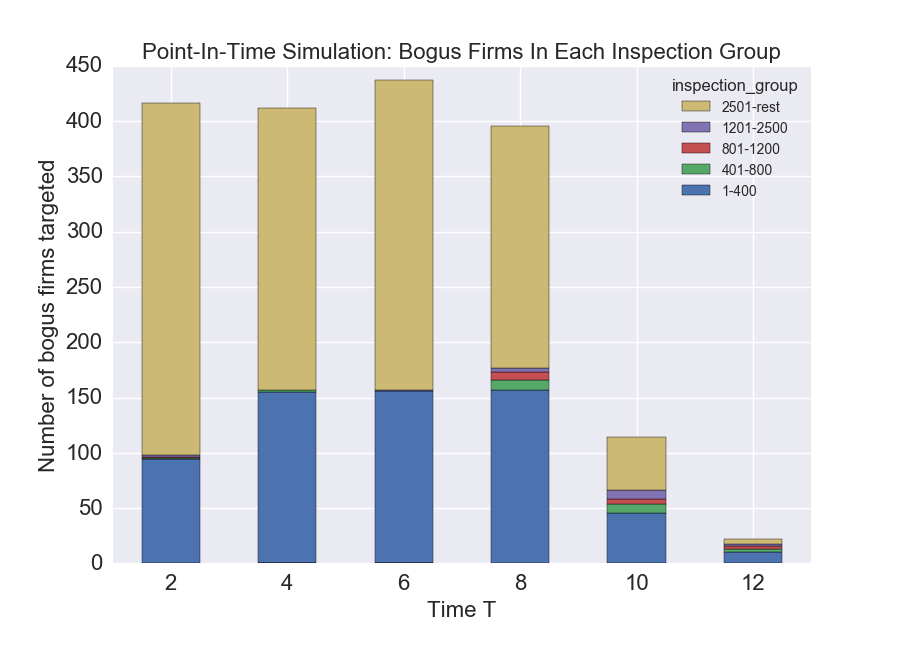
\includegraphics[width=0.4\textwidth]{figures/PointInTimePerformanceAggregate.png}
  \caption{Point-in-time simulations performance}
  \label{fig:PointInTimePerformanceArea}
  \floatfoot{\footnotesize For a point in time simulation in time T (x axis), out of all the bogus firms still operating, the chart shows the number of bogus firms that fall in each inspection group.}
 \end{figure}


\section{Future Work and Conclusion}
\label{sec:2-conclusion}
The purpose of this paper is to assess if a machine learning tool can be effective in catching bogus firms, in reducing the effort required by tax inspectors, and in eventually increasing tax collections. By creating a model from VAT returns from the state of Delhi, India and by analyzing the performance of the model, we provide evidence that targeting inspections based on a ML model could be highly beneficial even in a low compliance high evasion setting. Our results indicate that by using our tool the tax administration can prevent fraud up to \$15-45 million. Given that such data exists in many tax jurisdictions and that anecdotal evidence suggests that such false paper trails are a common problem, our work should have high policy relevance both within India and elsewhere.

The field level efficacy of the results that we have described in this paper needs to be investigated. We need to evaluate whether our work reduces the effort required by tax inspectors, and more importantly, does it improve revenue collections. A rigorous way to assess the reduction in administrative effort due to our model would be to target future inspections by comparing the recommendations of our model with a list of recommendations prepared by a team of tax officials and then inspecting the firms recommended by each and comparing performance. We are working with the Delhi tax authority to implement this.

Simultaneously, we aim to improve the results of our model by working closely with the tax authority in Delhi to conduct tax inspections on firms recommended by our model. We intend to stratify these inspections by our model score, inspecting firms throughout the model score distribution. Stratified inspection would provide a representative training set. On the other hand, inspecting the most likely bogus firms would provide more representatives from our rare class. We are not sure how to trade off those one vs. the other, but a similar point-in-time simulation exercise with our data where we only obtain information from our targeted inspections could shed light on this question.

Finally, recovering the revenue loss which can be directly attributed to bogus firms is not trivial. Often, the owners of these bogus firms can not be found at their declared addresses. Even if caught, they themselves have not benefited from the entire tax evasion. In fact, they have been key contributors to their trading partners who have managed to reduce their declared tax liability by interacting with these bogus firms. To do the actual revenue recovery, it is important to pursue the firms which interact with the bogus firms. Moreover, it is possible that even if the transactions that the trading partners declare with bogus firms have been canceled, the trading partners substitute these transactions to other yet to be identified bogus firms. If our system is deployed and bogus firms try to adapt, we will face a scenario of adversarial machine learning. All these are important questions which we hope to study as part of our future work.

%\section{Bibliography}
%\label{sec:bibliography}

%\bibliographystyle{plainnat}
%\bibliography{bib_chapter2}
